\section{Opacities}\label{sec:opac}
Radiative opacity is fundamental to stellar structure, it determines how much
incident radiation is absorbed or scattered. Moreover, when a media is in
thermodynamic equilibrium with the radiation field, that is when the temperature
of the media and that of the radiation field is the same, the opacity may be
used via Kirchhoff's law to find the emissivity of a material
\citep{Huebner2014}. Local Thermodynamic Equilibrium (LTE) is a common state to
find within a star and therefore stellar models have long relied on opacities
calculated in LTE.

\subsection{OPLIB Opacities}
Los Alamos National Labs OPLIB opacity tables were first computed in the 1990s
using the LEDCOP code \citep{Magee1995}; however, since 2004 efforts have been
underway to shift OPLIP from LEDCOP to ATOMIC \citep{Magee2004}. ATOMIC is a
LTE and non-LTE opacity and plasma modeling code. A major strength of ATOMIC
when compared to the older LEDCOP is its ability to vary its refinement level
\citep{Fontes2016}. For a more detailed breakdown of how the most up-to-date
set of OPLIB tables are generated see \citep{Colgan2016}.

The most up to date OPLIB tables include monochromatic Rosseland mean opacities
for elements hydrogen through zinc over temperatures 0.5eV to 100 keV and for
mass densities from approximately $10^{-8}$ g cm$^{-3}$ up to approximately
$10^{4}$ g cm$^{-3}$ (though the exact mass density range varies as a function
of temperature). The Rosseland mean opacity as reported in OPLIB tables is given
in Equation \ref{eqn:RMOATOMIC}.

\begin{align}\label{eqn:RMOATOMIC}
	\frac{1}{\kappa_{R}} =
		\frac{\int_{0}^{\infty}\frac{1}{\kappa_{\nu}}n_{\nu}^{3}\frac{\partial
		B_{\nu}}{\partial T}d\nu}{\int_{0}^{\infty}\frac{\partial B_{\nu}}{\partial
		T}d\nu}
\end{align}
Here, $B_{\nu}$ is the Planck function, $n_{\nu}$ is the frequency-dependent
refractive index \citep{Armstrong2014}, and $\kappa_{\nu}$ is the
frequency-dependent opacity. $\kappa_{\nu}$ is defined as the sum of the
bound-bound, bound-free, free-free, and scattering opacity computed by ATOMIC.

\subsection{Table Querying and Conversion}
DSEP uses pre-computed high-temperature opacity tables, in the format supplied
by OPAL. These tables list the Rosseland-mean opacity, $\kappa_{R}$, along
three dimensions: temperature, a density proxy R, and composition. R is defined
as
\begin{align} \label{eqn:Req}
	R = \frac{\rho}{T_{6}^{3}}
\end{align}
Where $T_{6} = T\times10^{-6}$ and $\rho$ is the mass density. If $T$ and
$\rho$ are given in cgs then for much of the radius of a star
$\log(R)\sim-1.5$.  The reason DSEP uses $R$ as opposed to simply tracking
opacity over density is that $R$ stays relatively fixed, whereas there is an
enormous dynamic range of densities within a star ($\sim 10^{5}$ [g cm$^{-3}$]
at the core of an RGB star all the way down to $\sim 10^{-8}$ [g
cm$^{-3}$] within the envelope). This reduction in
dynamic-range is important to help reduce floating-point numeric errors, which
ends up being the primary motivation to use $R$ over $\rho$.

OPLIB high-temperature opacity tables will replace the OPAL tables DSEP has used
since the release of the Dartmouth Stellar Evolution Database (DSED) in 2008
\citep{Dotter2008}. Just as OPAL tables were, OPLIB tables are queried from a
web interface\footnote{https://aphysics2.lanl.gov/apps/}. So that we might
generate many tables easily and quickly we develope a web scraper built with
Python's \texttt{requests} module in addition to the 3rd party
\texttt{mechanize} and \texttt{BeautifulSoup} modules \citep{chandra2015python,
richardson2007beautiful} which can get tables with minimal human intervention.
This web scraper submits a user requested chemical composition (composed of
mass fractions for elements from Hydrogen to Zinc) to the Los Alamos web form, selects
0.0005 keV as the lower temperature bound and 60 keV as the upper temperature
bound, and finally requests opacity measurements for 100 densities, ranging
from $1.77827941\times 10 ^{-15}$ [g cm$^{-3}$] up to $1\times10^{7}$ [g
cm$^{-3}$], at each temperature interval. These correspond to approximately the
same temperature and density range of opacities present in the OPAL opacity
tables.

So as not to break compatibility with OPAL tables we create a translation layer
to convert OPLIB tables to OPAL format. This allows for transparent use of the new
tables without any direct modifications to the DSEP source. The primary job of
this translation layer is to unit conversion, secondarily the structure of OPAL
tables must be matched byte-for-byte.

OPLIB reports $\kappa_{R}$ as a function of mass density, temperature in keV,
and composition. Recall that OPAL tables present opacity as a function of
temperature in Kelvin, $R$, and composition. The conversion from temperature
in keV to Kelvin is trivial
\begin{align}
	T_{K} = T_{keV} * 11604525.0061657
\end{align}
The conversion from mass density to $R$ is more involved. Because $R$ is
coupled with both mass density and temperature there there is no way to
directly convert tabulated values of opacity reported in the OPLIB tables to
their equivalents in $R$ space. Instead we must rotate the tables,
interpolating $\kappa_{R}(\rho,T_{eff}) \rightarrow \kappa_{R}(R,T_{eff})$. 

As a first step in this rotation we use the \texttt{interp2d} function within
\texttt{scipy}'s \texttt{interpolate} \citep{2020SciPy-NMeth} module to
construct a cubic bivariate B-spline \citep{Dierckx1981} interpolating function
$s$, with a smoothing factor of 0, representing the surface $\kappa_{R}(\rho,
T_{eff})$. For each $R^{i}$ and $T^{j}_{eff}$ which DSEP expects
high-temperature opacities to be reported for, we evaluate Equation
\ref{eqn:Req} to find $\rho^{ij} = \rho(T^{j}_{eff},R^{i})$.  Opacities in
$T_{eff}$, $R$ space are then inferred as $\kappa^{ij}_{R}(R^{i},T^{j}_{eff}) =
s(\rho^{ij}, T^{j}_{eff})$. Finally, some number of upper-left and lower-right
hand entries in each table are discarded as DSEP takes non rectangular tables
as input, the exact number and indices of the discarded entries is dependent
on composition.

As first-order validation of this interpolation scheme we can preform a similar
interpolation in the opposite direction, rotating the tables back to
$\kappa_{R}(\rho, T_{eff})$ and then comparing the initial, ``raw'', opacities
to those which have gone through the interpolations process. Figure
\ref{fig:fracdiff} shows the fractional difference between the raw opacities
and a set which have gone through this double interpolation. The red line
denotes $Log(R)=-1.5$ where models will tend to sit for much of their radius.
Along the $Log(R)=-1.5$ line the mean fractional difference is $\langle \delta
\rangle = 0.006$ with an uncertainty of $\sigma_{\langle\delta\rangle} =
0.009$. One point of note is that, because the initial rotation into $Log(R)$
space also reduces the domain of the opacity function interpolation-edge
effects which we avoid initially by extending the domain past what DSEP needs
cannot be avoided when interpolating back into $\rho$ space. In future, a more
robust validation, which does not reduce the domain size will be conducted.

\begin{figure}
	\centering
	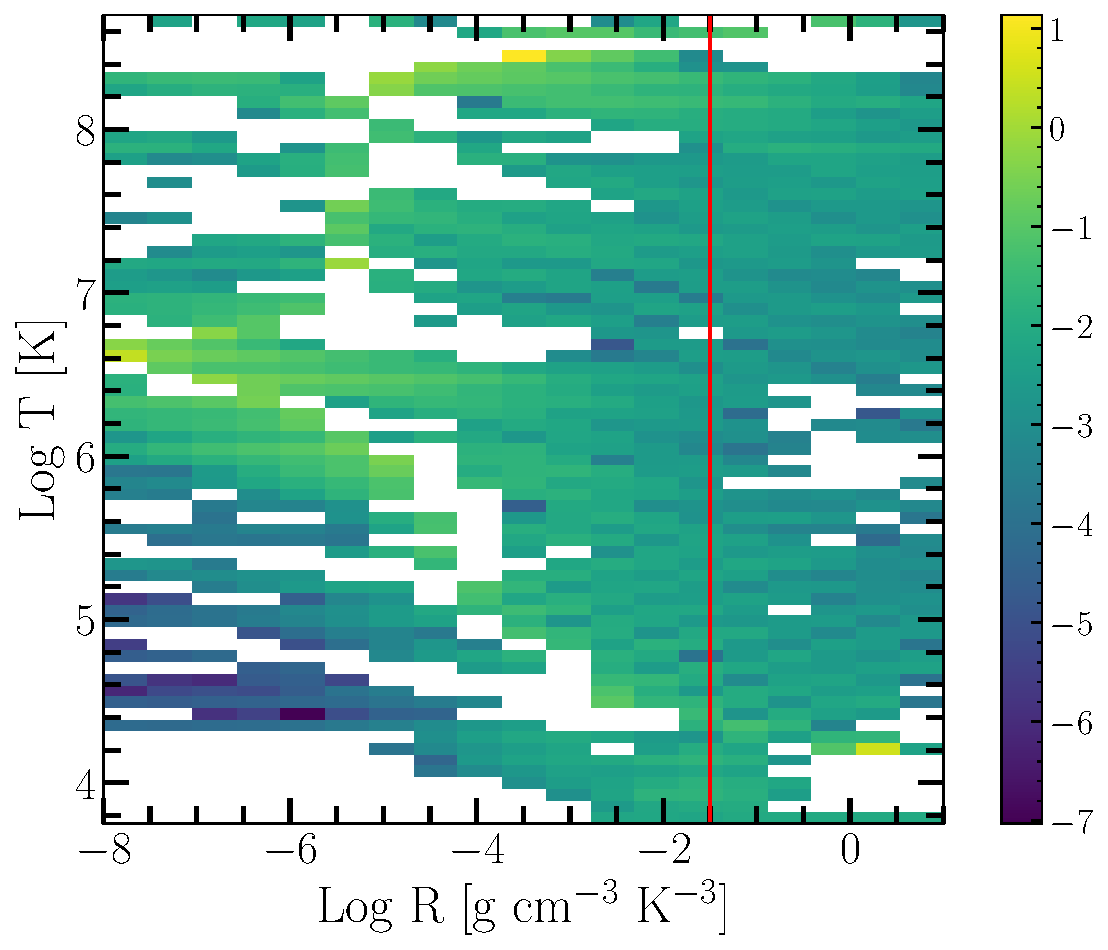
\includegraphics[width=0.45\textwidth]{src/figures/FractionalDifference.pdf}
	\caption{Log Fractional Difference between opacities in $\kappa_{R}(\rho,
	T_{eff})$ space directly queried from the OPLIB webform and those which
	have been interpolated into $Log(R)$ space and back. Note that, due to the
	temperature grid DSEP uses not aligning perfectly which the temperature
	grid OPLIB uses there may be edge effects where the interpolation is poorly
	constrained. The red line corresponds to $Log(R) = -1.5$ where much of a
	stellar model's radius exists.}
	\label{fig:fracdiff}
\end{figure}

\subsection{Opacity Validation}
In order to further validate the OPLIB high-temperature opacities we first visually
compare a set of opacity vs. temperature curves from OPLIB at a constant $R$
and \citet{Grevesse1998} composition (GS98) to the same curve from OPAL. A
characteristic opacity vs temperature curve is shown in Figure
\ref{fig:OpacCompare}, $\log _{10}(R) = -1.5$ is chosen as for much of the
radius of a main sequence star $\log _{10}(R)$ is around that value. The
largest variation in $\kappa_{R}$ from OPAL to OPLIB at $\log _{10}(R)=-1.5$ is
on the order of a few percent. This is inline with expectations of OPLIB and OPAL
being in relatively close agreement \citep{Colgan2016}.

\begin{figure}
	\centering
	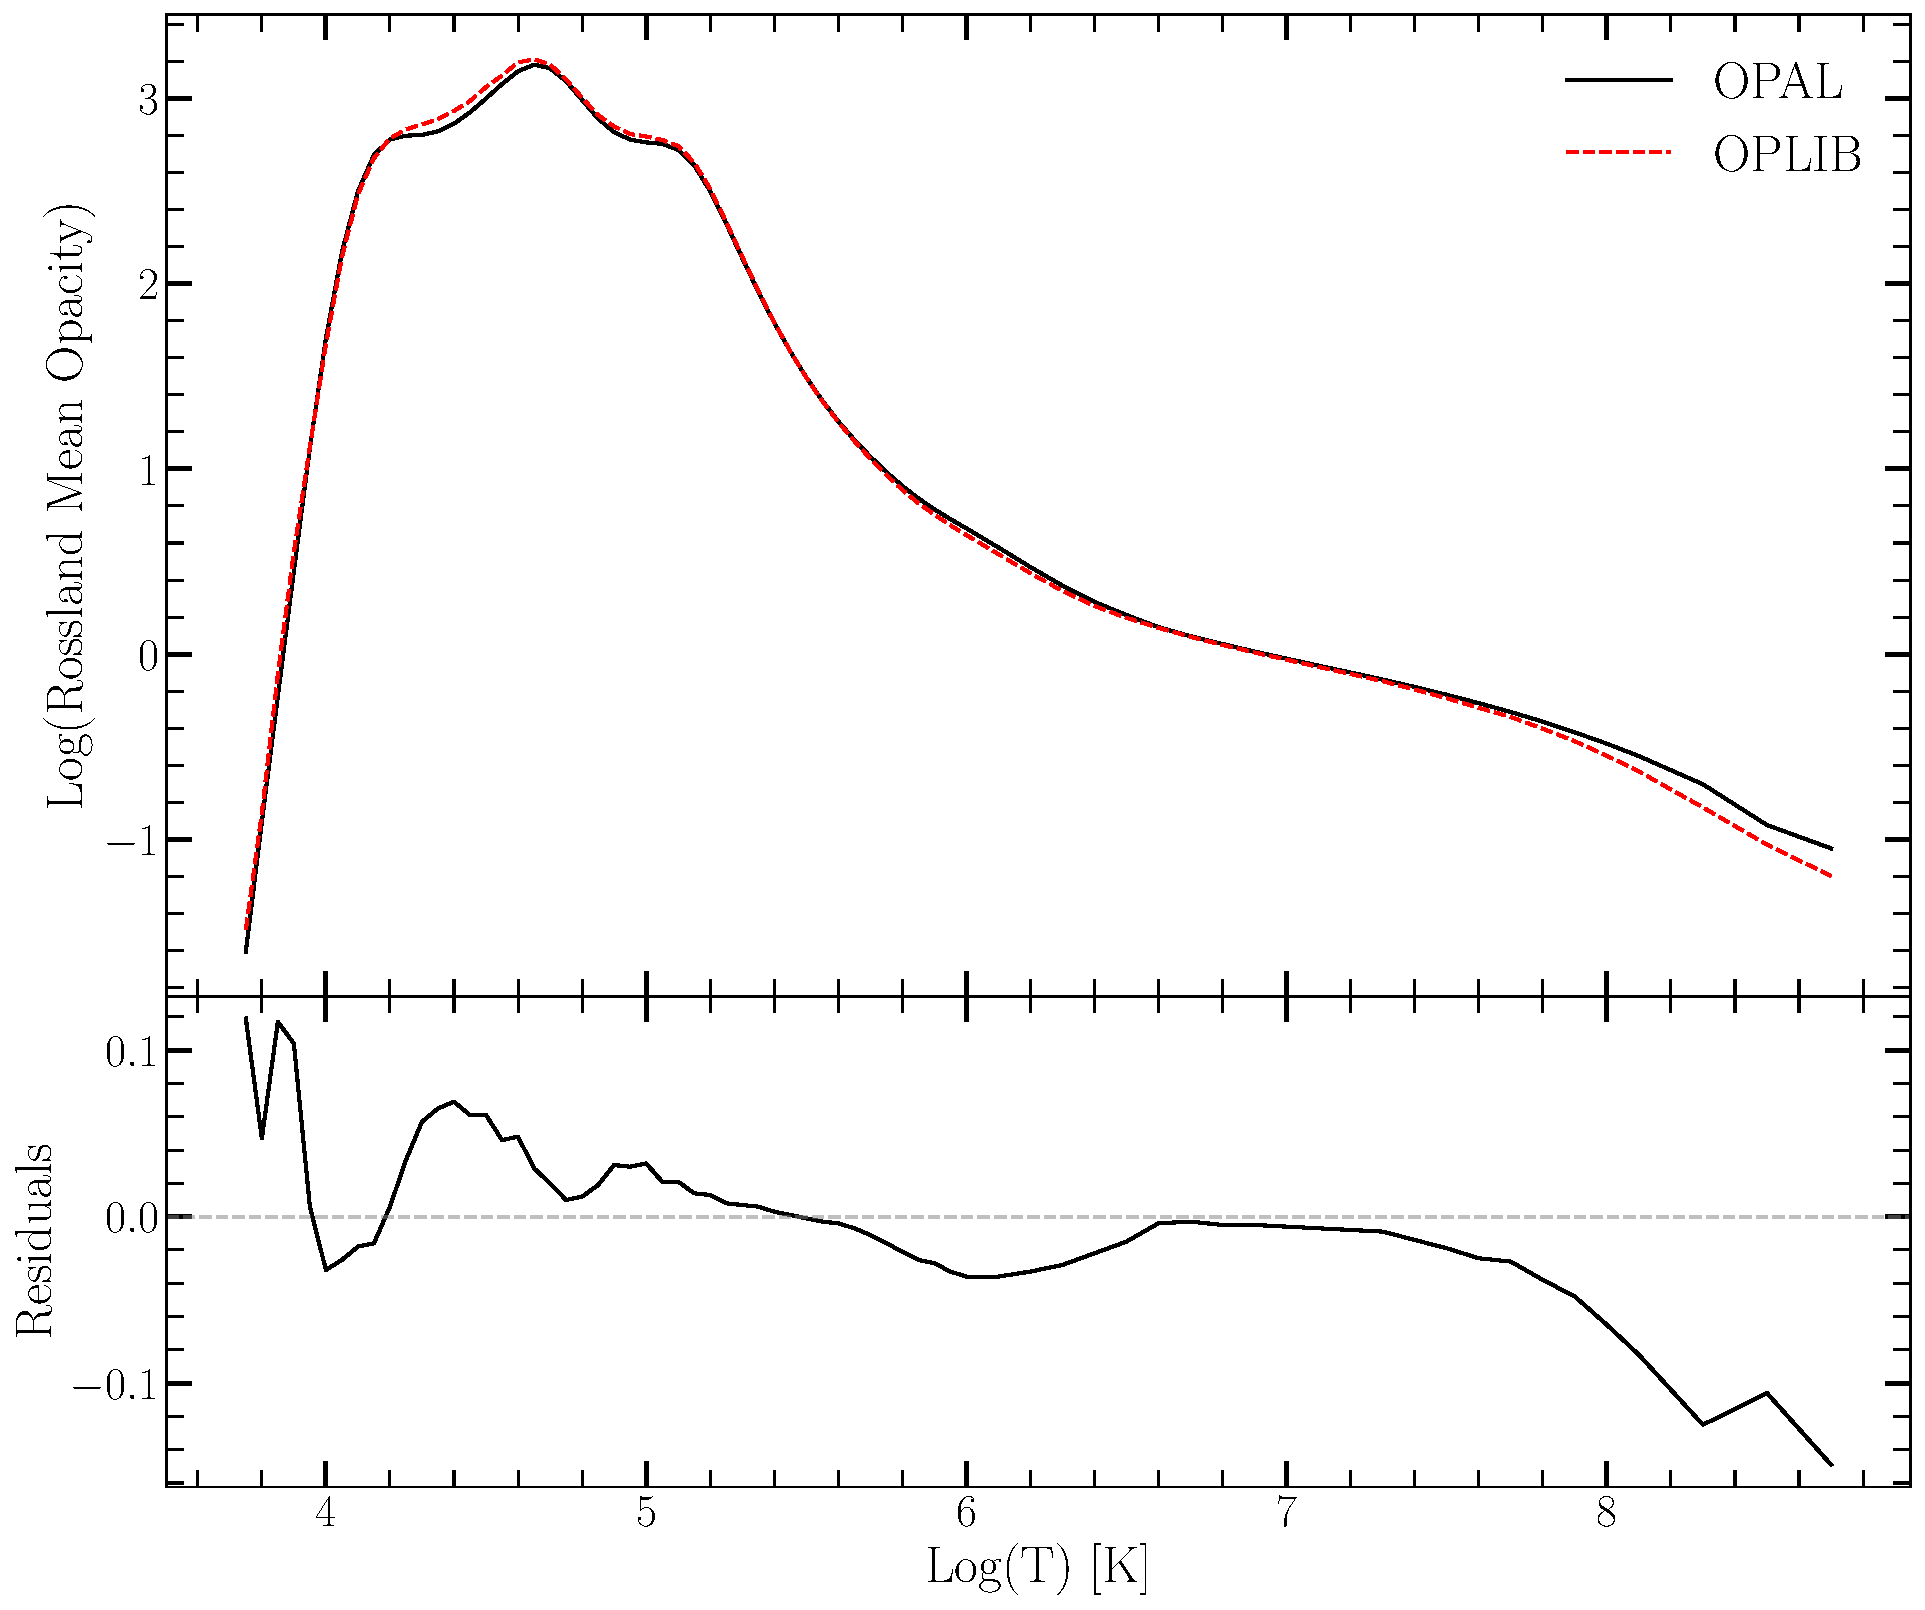
\includegraphics[width=0.45\textwidth]{src/figures/OpacityComparision.pdf}
	\caption{Rosseland mean opacity with the GS98 solar composition for both
		OPAL opacities and OPLIB opacities (top). Residuals between OPLIB
		opacities and OPAL opacities (bottom). These opacities are plotted at
		$\log _{10}(R) = -1.5$, $X=0.7$, and $Z=0.02$.}
	\label{fig:OpacCompare}
\end{figure}

To further validate the OPLIB opacities we generate a solar calibrated stellar
model (SCSM) using the new tables. SCSMs are generally models where some
initial parameters have been iteratively adjusted to minimize some loss function
between that models output parameters and the observed values of those
parameters for the Sun. In the context of this paper we adjust both the
convective mixing length parameter, $\alpha_{ML}$, and the initial Hydrogen
mass fraction, $X$, to minimize the difference between the models final radius
and luminosity and that of the sun.

Optimization of $\alpha_{ML}$ and $X$ is done with a quite naive gradient
descent algorithm. For each optimization step three models are evolved: a reference
model, a model with a small perturbation to the hydrogen mass fraction but the
same mixing length as the reference model, and a model with a small
perturbation to the mixing length but the same hydrogen mass fraction as the
reference. Perturbations are sampled from a normal distribution (implemented
though \texttt{numpy.random}) with scale set to an adjustable parameter,
$\eta$. This distribution is sampled and that sample is then added to the
reference value for either $X$ or $\alpha_{ML}$. The luminosity and radius of
the three evolved models are compared to solar values and the gradient of the
resultant $L-L_{\odot}$, $R-R_{\odot}$ surface is followed down to new
estimates for the reference values of $X$ and $\alpha_{ML}$. This process is
is repeated until the difference between successive $X$ and $\alpha_{ML}$ drops
below one part in $10^{5}$.

\begin{figure}
	\centering
	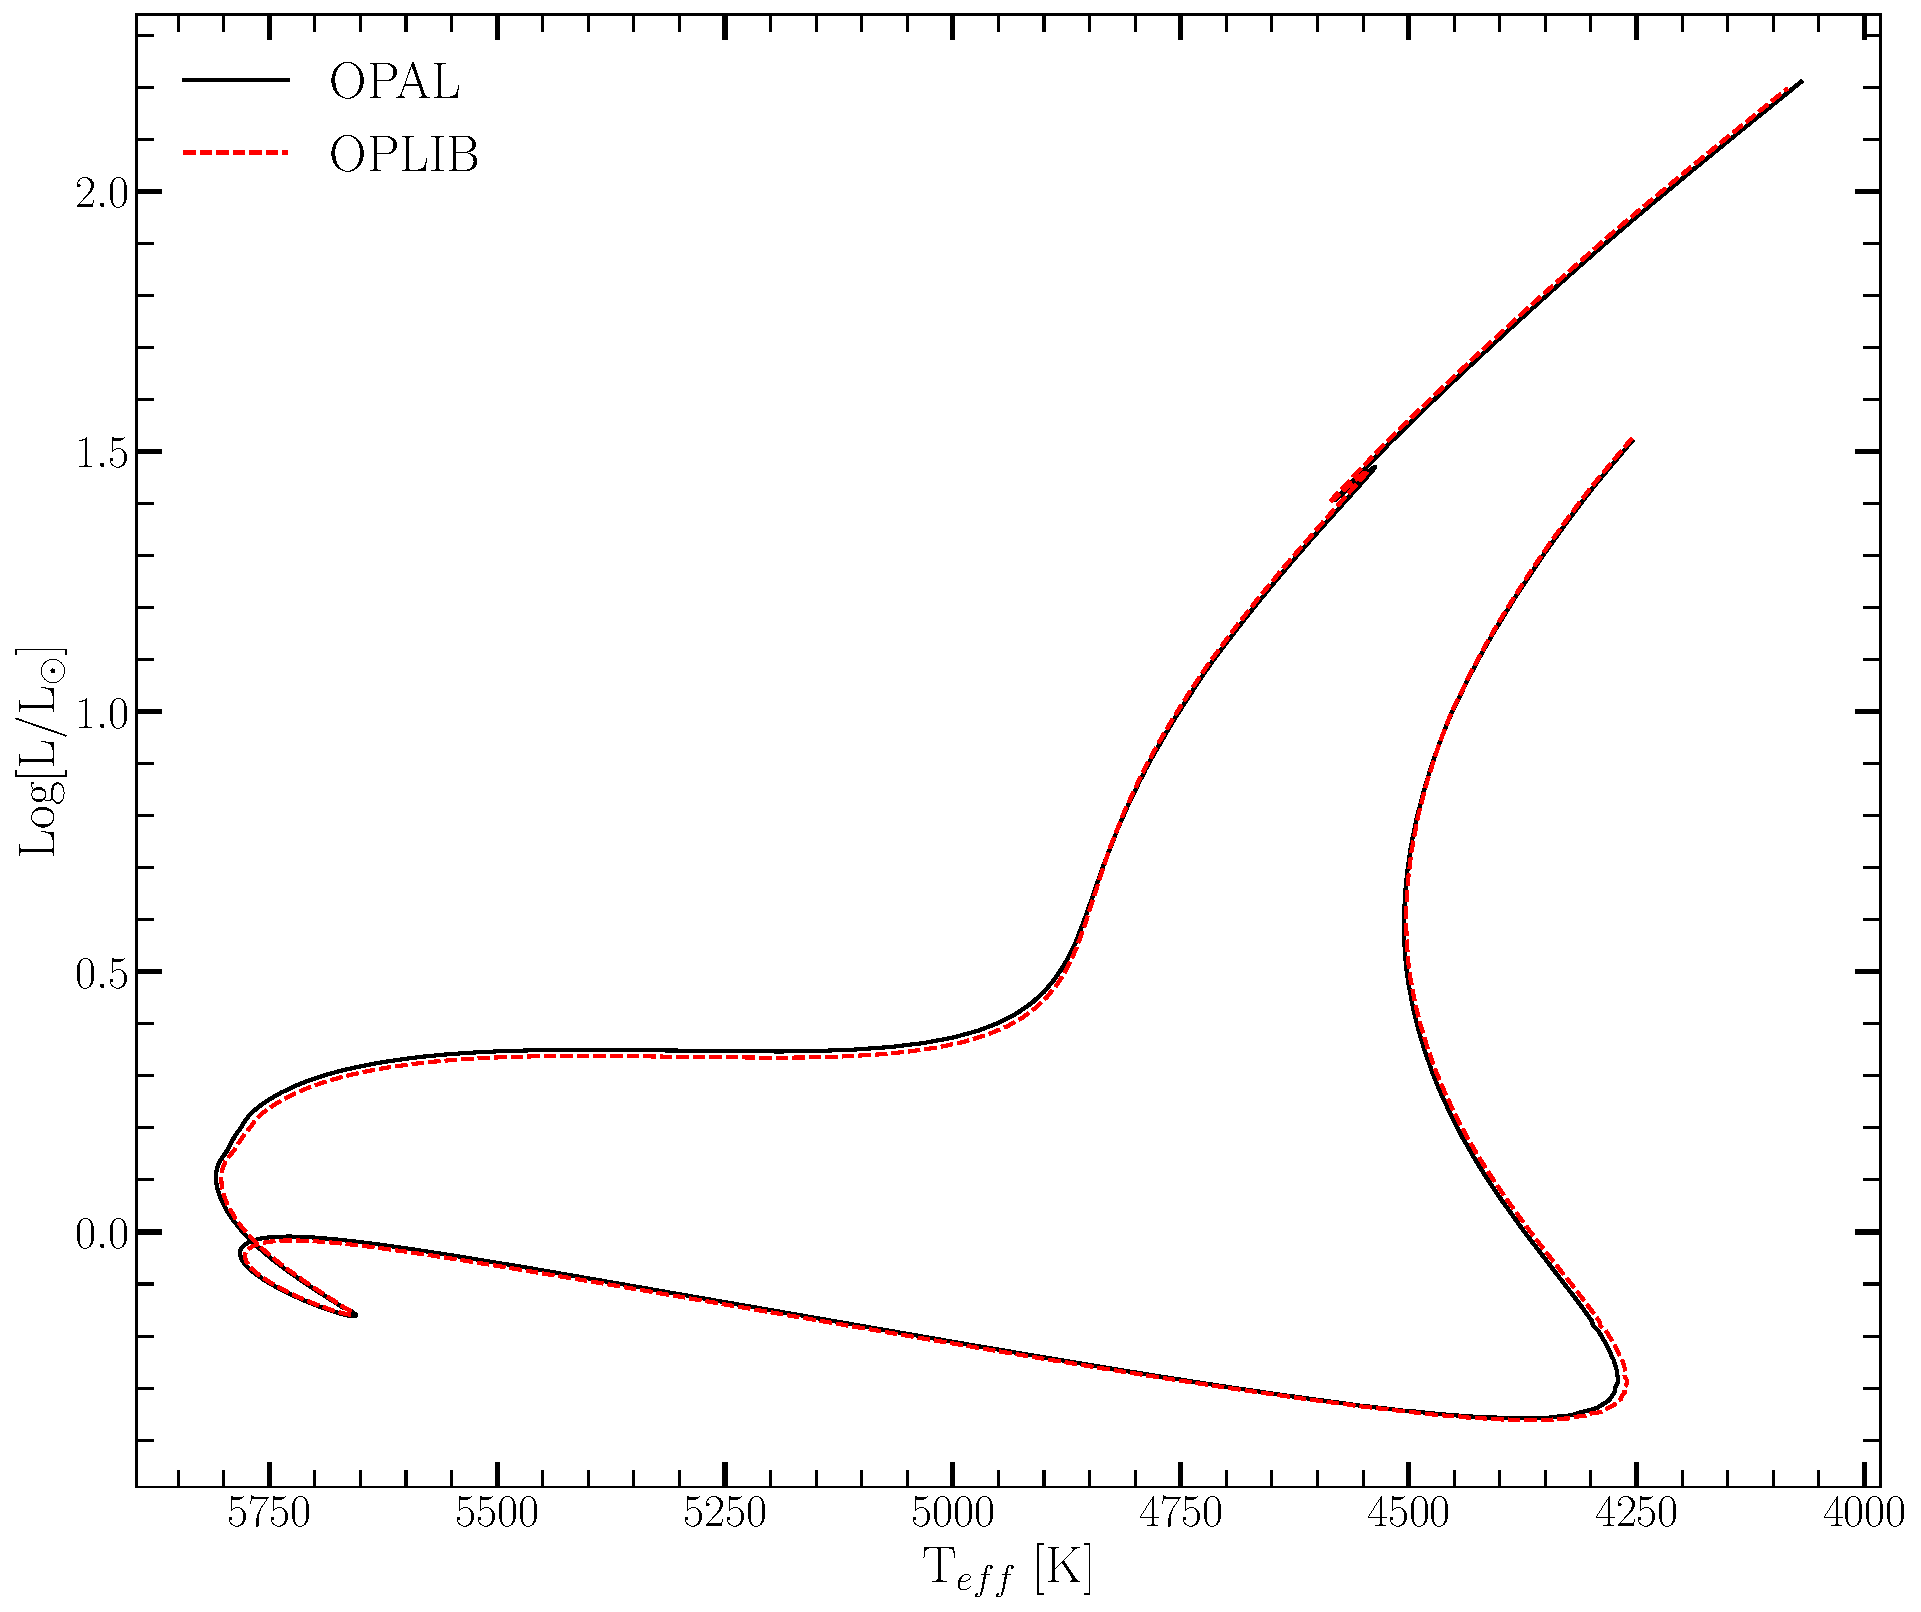
\includegraphics[width=0.45\textwidth]{src/figures/HRDiagramOPALvsOPLIB_SCCM.pdf}
	\caption{HR Diagram for the two SCSMs, OPAL and OPLIB. OPLIB is show as a grey
	dashed line.}
	\label{fig:OPLIBOPALHR}
\end{figure}

If we generate a SCSM using the GS98 OPAL opacity tables we find a best
estimate of $X=0.7066$ and $\alpha_{ML} = 1.9333$. When we preform the same
calibration but substituting in the GS98 OPLIB tables we find $X=0.7107$ and
$\alpha_{ML} = 1.9629$. This represents $\sim 0.5\%$ difference in the SCSM
hydrogen mass fractions and $\sim 1.5\%$ change in the SCSM convective mixing
length parameters when comparing models using OPAL and OPLIB tables. An
HR-diagram for the two calibrated models is presented in Figure
\ref{fig:OPLIBOPALHR}. While the two evolutionary tracks are very similar, note
that the OPLIB SCSM's luminosity is systematically lower at the same effective
temperature all the way from the premain sequence up and until the star leaves
the main sequence, at which point it is effectively the same as the OPAL SCSM.
This luminosity difference between OPAL and OPLIB based models is consistent
with expectations given the differences in opacities. Opacity is of primary
importance only in radiative regions of a star ($\gtrsim 10^{6}$ K). Figure
\ref{fig:OpacCompare} shows that OPLIB opacities are uniformly lower than OPAL
opacities above $10^{6}$ K. These lower opacities will steepen the temperature
gradient within the stellar model as radiation streams more freely outward.
